\documentclass[notheorems,hidelinks,aspectratio=1610]{beamer}
%\usetheme[compress]{JuanLesPins}
\usetheme{JuanLesPins}
\usecolortheme{iwr}
\usepackage{mathsim}
\lstset{language=Python}
\usetikzlibrary{snakes}
\usetikzlibrary{matrix,fit}
\pgfdeclarelayer{bg}
\pgfsetlayers{bg,main}
\tikzset{velox/.style={color=black,draw,fill=red,thick,%
    shape=diamond,aspect=.4,
    inner sep=1.3pt,transform shape}}
\tikzset{veloy/.style={color=black,draw,fill=red,thick,%
    shape=diamond,aspect=2.5,
    inner sep=1.3pt,transform shape}}
\tikzset{veloxy/.style={color=black,draw,fill=red,thick,%
    shape=star,star points=4,star point ratio=2.2,
    inner sep=1.3pt,transform shape}}
\tikzset{pressure/.style={color=black,draw,fill=cyan,thick,%
    shape=circle,inner sep=2pt,transform shape}}
\tikzset{velo/.style={transform shape,double=red,arrows={-Stealth[open,fill=red]}}}

%% Macros for drawing degrees of freedom for different shapes/elements.
%% Arguments are always:
%%   #1: Starting point
%%   #2: End point
%%   #3: polynomial degree
%%   #4: node settings

\tikzset{pics/edgenormal/.style args={#1/#2/#3/#4}{%
    code={%
      \draw #1 -- #2
      node foreach \x [evaluate=\x as \xval] in {1,...,#3} [#4,sloped,pos=\xval/(#3+1)] {};
      }
}}


%% Macros for drawing degrees of freedom for different shapes/elements.
%% Arguments are always:
%%   #1: polynomial degree
%%   #2: node settings

\tikzset{pics/tripile/.style args={#1/#2}{%
    code={%
      \coordinate (top) at (0,#1);
      \foreach \i in{0,...,#1}
      \foreach \j in{0,...,\i}
      {
        \tikzmath{
          \y = .3*(2/3*#1-\i)*cos(30);
          \x = .3*(\i/2-\j);
        }
        \node[#2] at (\x,\y) {};
      }
    }
}}

\tikzset{pics/tensor/.style args={#1/#2/#3}{%
    code={%
      \coordinate (top) at (0,#1);
      \foreach \i in{0,...,#1}
      \foreach \j in{0,...,#2}
      {
        \tikzmath{
          \y = 2*(\i+1)/(#1+2);
          \x = 2*(\j+1)/(#2+2);
        }
        \node[#3] at (\x,\y) {};
      }
    }
}}

\tikzset{pics/pfem/.style args={#1/#2}{%
    code={%
      \tikzmath{ \ytop=2*cos(30); }
      \coordinate (top) at (0,\ytop);

      \foreach \i in{0,...,#1}
      \foreach \j in{0,...,\i}
      {
        \tikzmath{
          \y = \ytop-\ytop*\i/#1;
          \x = 2*(\i/2-\j)/#1+1;
        }
        \node[#2] at (\x,\y) {};
      }
    }
}}

\tikzset{pics/qfem/.style args={#1/#2}{%
    code={%
      \foreach \i in{0,...,#1}
      \foreach \j in{0,...,#1}
      {
        \tikzmath{
          \y = 2-2*\i/#1;
          \x = 2-2*\j/#1;
        }
        \node[#2] at (\x,\y) {};
      }
    }
}}

%%% Local Variables:
%%% mode: latex
%%% TeX-master: "all"
%%% End:

\def\esp#1{V_{#1}}

\usepackage{times}
\usepackage{xr}
\externaldocument{main}
\usepackage{mfirstuc}
\usepackage{mathtools}  
\mathtoolsset{showonlyrefs}

\newcommand{\rd}{\operatorname{rd}}

\def\footnote#1{}
\def\putindex#1{#1}
\title{Numerical Linear Algebra}
\author{Guido Kanschat}
\date{\today}

\input{slides-only}

\begin{document}
\frame{\maketitle}
\frame{\frametitle{Overview}\tableofcontents[hideallsubsections]}

%%%%%%%%%%%%%%%%%%%%%%%%%%%%%%%%%%%%%%%%%%%%%%%%%%%%%%%%%%%%%%%%%%%%%%
%%%%%%%%%%%%%%%%%%%%%%%%%%%%%%%%%%%%%%%%%%%%%%%%%%%%%%%%%%%%%%%%%%%%%%
\section{Orthogonalization and QR Factorization}
%%%%%%%%%%%%%%%%%%%%%%%%%%%%%%%%%%%%%%%%%%%%%%%%%%%%%%%%%%%%%%%%%%%%%%
%%%%%%%%%%%%%%%%%%%%%%%%%%%%%%%%%%%%%%%%%%%%%%%%%%%%%%%%%%%%%%%%%%%%%%
\subsection{The Gram-Schmidt algorithm}
\frame{\sectoc}

\frame {\input {blocks/Algorithm-gram-schmidt.tex}
  \input {blocks/Theorem-gram-schmidt.tex}}

\frame {\input {blocks/Algorithm-gram-schmidt-implementation.tex}}
\frame {\input {blocks/Problem-gram-schmidt-implementation.tex}}

\frame {\input {blocks/Notation-column-vectors.tex}}
\frame {\input {blocks/Notation-matrix-linear-combination.tex}}

\frame {\input {blocks/Definition-qr-decomposition.tex}}
\frame {\input {blocks/Lemma-qr-columns.tex}
  \input {blocks/Theorem-qr-existence.tex}}

%%%%%%%%%%%%%%%%%%%%%%%%%%%%%%%%%%%%%%%%%%%%%%%%%%%%%%%%%%%%%%%%%%%%%%
\subsection{Householder reflection}
\frame{\subtoc}
%%%%%%%%%%%%%%%%%%%%%%%%%%%%%%%%%%%%%%%%%%%%%%%%%%%%%%%%%%%%%%%%%%%%%%

\frame {\input {blocks/Definition-householder-transformation.tex}}
\frame {\input {blocks/Lemma-householder-symmetry.tex}}
\frame {\input {blocks/Lemma-householder-qr.tex}}
\frame {\input {blocks/Notation-colon-notation.tex}}
\frame {\input {blocks/Problem-householder-compute.tex}}
\frame {\input {blocks/Algorithm-householder-multiplication.tex}}
\frame {\input {blocks/Problem-householder-product.tex}}

%%%%%%%%%%%%%%%%%%%%%%%%%%%%%%%%%%%%%%%%%%%%%%%%%%%%%%%%%%%%%%%%%%%%%%
\subsection{Givens rotation}
\frame{\subtoc}
%%%%%%%%%%%%%%%%%%%%%%%%%%%%%%%%%%%%%%%%%%%%%%%%%%%%%%%%%%%%%%%%%%%%%%

\frame {\input {blocks/Definition-givens.tex}}
\frame {\input {blocks/Lemma-givens-computation.tex}}
\frame {\input {blocks/Notation-givens-specific.tex}}
\frame {\input {blocks/Algorithm-givens-computation.tex}}
\frame {\input {blocks/Definition-givens-complex.tex}}
\frame {\input {blocks/Lemma-givens-computation-complex.tex}}
\frame {\input {blocks/Lemma-givens-computation-complex-2.tex}}
\frame {\input {blocks/Algorithm-givens-multiplication.tex}}


%%% Local Variables:
%%% mode: latex
%%% TeX-master: "slides"
%%% End:


%%%%%%%%%%%%%%%%%%%%%%%%%%%%%%%%%%%%%%%%%%%%%%%%%%%%%%%%%%%%%%%%%%%%%%
%%%%%%%%%%%%%%%%%%%%%%%%%%%%%%%%%%%%%%%%%%%%%%%%%%%%%%%%%%%%%%%%%%%%%%
\section{Dense Algebraic Eigenvalue Problems}
\frame{\sectoc}
%%%%%%%%%%%%%%%%%%%%%%%%%%%%%%%%%%%%%%%%%%%%%%%%%%%%%%%%%%%%%%%%%%%%%%
%%%%%%%%%%%%%%%%%%%%%%%%%%%%%%%%%%%%%%%%%%%%%%%%%%%%%%%%%%%%%%%%%%%%%%
\subsection{Mathematical background}
\subsubsection{Definition of EVP}
\frame{\subsubtoc}
\frame {\input {blocks/Definition-eigenvalue.tex}}
\frame {\input {blocks/Definition-eigenvalue-algebraic.tex}
  \pause
  \input {blocks/Lemma-eigenvalue-equivalent.tex}}
\frame {\input {blocks/Theorem-eigenvalue-count.tex}
  \pause
  \input {blocks/Definition-eigenvalue-simple.tex}}
\frame {\input {blocks/Definition-right-left-ev.tex}
\input {blocks/Lemma-eigenvalues-conjugate.tex}}
\frame {\input {blocks/Definition-invariant-subspace.tex}}
\frame {\input {blocks/Theorem-invariant-eigenvalues.tex}}
\frame {\input {blocks/Definition-spectral-projector.tex}}
\frame {\input {blocks/Definition-dominant_ev.tex}}

\subsubsection{Bases and matrices}
\frame{\subsubtoc}
\frame {\input {blocks/Lemma-change-of-basis.tex}}
\frame {\input {blocks/Corollary-change-of-basis.tex}}
\frame {\input {blocks/Definition-similar-matrix.tex}
  \input {blocks/Lemma-similarity-equivalence.tex}}
\frame {\input {blocks/Lemma-matrix-basis-change.tex}}
\frame {\input {blocks/Theorem-Jordan-canonical-form.tex}}
\frame {\input {blocks/Definition-diagonalizable.tex}
  \input {blocks/Theorem-matrix-functions.tex}}
\frame {\input {blocks/Theorem-simultaneous-diagonalization.tex}}

% Move this!
\frame {\input {blocks/Lemma-similarity-eigenvalues.tex}}

\subsubsection{The Schur canonical form}
\frame{\subsubtoc}

\frame {\input {blocks/Theorem-schur-canonical.tex}
  \input {blocks/Lemma-schur-canonical-1.tex}}
\frame {\input {blocks/Lemma-schur-canonical-2.tex}
  \input {blocks/Definition-dominant-invariant-subspace.tex}}

\subsubsection{Normal and Hermitian matrices}
\frame{\subsubtoc}

\frame {\input {blocks/Definition-sesqui.tex}}
\frame {\input {blocks/Definition-inner-product.tex}
  \input {blocks/Example-Euclidean-ip.tex}}
\frame {\input {blocks/Definition-conjugate-matrix.tex}}
\frame {\input {blocks/Definition-orthonormal-unitary.tex}}

\frame {\input {blocks/Definition-normal-Hermitian.tex}}
\frame {\input {blocks/Lemma-Hermitian-eigenvalues-real.tex}
\input {blocks/Theorem-Hermitian-diagonalizable.tex}
\input {blocks/Corollary-symmetric-diagonalizable.tex}}
\frame {\input {blocks/Lemma-normal-properties.tex}}
\frame {\input {blocks/Theorem-normal-diagonalizable.tex}}

%%% Local Variables:
%%% mode: latex
%%% TeX-master: "slides"
%%% End:

%%%%%%%%%%%%%%%%%%%%%%%%%%%%%%%%%%%%%%%%%%%%%%%%%%%%%%%%%%%%%%%%%%%%%%
\subsection{Well-posedness and bounds}
\frame{\subtoc}
%%%%%%%%%%%%%%%%%%%%%%%%%%%%%%%%%%%%%%%%%%%%%%%%%%%%%%%%%%%%%%%%%%%%%%
\subsubsection{Conditioning of the EVP}

\frame {\input {blocks/Definition-matrix-norm.tex}}
\frame {\input {blocks/Lemma-bound-by-norm.tex}}
\frame {\input {blocks/Lemma-pre-gershgorin.tex}}

\frame {\input {blocks/Definition-conditioning-eigenvalue.tex}}
\frame {\input {blocks/Example-characteristic-polynomial.tex}}
\frame {\input {blocks/Example-conditioning-Jordan-block.tex}}
\frame {\input {blocks/Theorem-Jordan-block-ill-conditioned.tex}}
\frame {\input {blocks/Theorem-bauer-fike.tex}
  \only<1>{\input {blocks/Definition-matrix-condition.tex}}
  \only<2>{\input {blocks/Corollary-conditioning-eigenvalues-normal.tex}}}
\frame {\input {blocks/Theorem-conditioning-eigenvalue-single.tex}}
\frame {\input {blocks/Theorem-eigenvalues-continuous.tex}}

\subsubsection{Conditioning of eigenvectors}

\frame {\input {blocks/Example-conditioning-eigenvectors.tex}
  \pause
  \input {blocks/Remark-conditioning-eigenvectors.tex}}
\frame {\input {blocks/Problem-almost-parallel.tex}}

\subsubsection{Bounds on eigenvalues}
\frame {\input {blocks/Theorem-gershgorin.tex}}
\subsubsection{The Rayleigh quotient}
\frame {\input {blocks/Definition-rayleigh-quotient.tex}}
\frame {\input {blocks/Theorem-minmax.tex}}
\frame {\input {blocks/Lemma-Rayleigh-approximation.tex}}

%%% Local Variables:
%%% mode: latex
%%% TeX-master: "slides"
%%% End:

%%%%%%%%%%%%%%%%%%%%%%%%%%%%%%%%%%%%%%%%%%%%%%%%%%%%%%%%%%%%%%%%%%%%%%
\subsection{Vector iterations}
\frame{\subtoc}
%%%%%%%%%%%%%%%%%%%%%%%%%%%%%%%%%%%%%%%%%%%%%%%%%%%%%%%%%%%%%%%%%%%%%%
\frame {\input {blocks/Algorithm-vector-iteration.tex}}
\frame {\input {blocks/Theorem-vector-iteration.tex}}
\frame {\input {blocks/Remark-vector-iteration.tex}}
\frame {\input {blocks/Lemma-Rayleigh-approximation.tex}}
\frame {\input {blocks/Algorithm-vector-iteration-rayleigh.tex}}
\frame {\input {blocks/Remark-vector-iteration.tex}}
\frame {\input {blocks/Remark-vector-iteration-roundoff.tex}}

\frame {\input {blocks/Algorithm-shifted-vector-iteration.tex}}
\frame {\input {blocks/Definition-shifted-matrix-polynomial.tex}
  \input {blocks/Lemma-matrix-polynomial.tex}}
\frame {\input {blocks/Algorithm-polynomial-filtering.tex}}
\frame {\input {blocks/Example-polynomial-filtering.tex}}
\frame {\input {blocks/Algorithm-vector-iteration-polynomial.tex}}

\frame {\input {blocks/Algorithm-subspace-iteration.tex}}
\frame {\input {blocks/Theorem-convergence-subspace-iteration.tex}}
\frame {\input {blocks/Definition-projection-distance.tex}
  \input {blocks/Example-projection-distance.tex}}
\frame {\input {blocks/Corollary-convergence-subspace-iteration.tex}}

%%% Local Variables:
%%% mode: latex
%%% TeX-master: "slides"
%%% End:

%%%%%%%%%%%%%%%%%%%%%%%%%%%%%%%%%%%%%%%%%%%%%%%%%%%%%%%%%%%%%%%%%%%%%%
\subsection{Vector iterations}
\frame{\subtoc}
%%%%%%%%%%%%%%%%%%%%%%%%%%%%%%%%%%%%%%%%%%%%%%%%%%%%%%%%%%%%%%%%%%%%%%
\frame {\input {blocks/Algorithm-vector-iteration.tex}}
\frame {\input {blocks/Theorem-vector-iteration.tex}}
\frame {\input {blocks/Remark-vector-iteration.tex}}
\frame {\input {blocks/Lemma-Rayleigh-approximation.tex}}
\frame {\input {blocks/Algorithm-vector-iteration-rayleigh.tex}}
\frame {\input {blocks/Remark-vector-iteration.tex}}
\frame {\input {blocks/Remark-vector-iteration-roundoff.tex}}

\frame {\input {blocks/Algorithm-shifted-vector-iteration.tex}}
\frame {\input {blocks/Definition-shifted-matrix-polynomial.tex}
  \input {blocks/Lemma-matrix-polynomial.tex}}
\frame {\input {blocks/Algorithm-polynomial-filtering.tex}}
\frame {\input {blocks/Example-polynomial-filtering.tex}}
\frame {\input {blocks/Algorithm-vector-iteration-polynomial.tex}}

\frame {\input {blocks/Algorithm-subspace-iteration.tex}}
\frame {\input {blocks/Theorem-convergence-subspace-iteration.tex}}
\frame {\input {blocks/Definition-projection-distance.tex}
  \input {blocks/Example-projection-distance.tex}}
\frame {\input {blocks/Corollary-convergence-subspace-iteration.tex}}

\subsection{The QR-iteration}

\subsubsection{Definition and basic properties}
\frame{\subsubtoc}

\frame {\input {blocks/Algorithm-qr-iteration.tex}
  \input {blocks/Lemma-qr-1.tex}}

\subsubsection{Implementation issues}
\frame{\subsubtoc}

\frame {\input {blocks/Definition-hessenberg.tex}}
\frame {\input {blocks/Algorithm-Hessenberg-qr.tex}}

\begin{frame}
  \frametitle{Example: 4-by-4-matrix}
  \begin{gather*}
    \matH \to \givens_{12}^*\matH
    \visible<2->{\to \givens_{23}^*\givens_{12}^*\matH}
    \visible<3->{\to \givens_{34}^*\givens_{23}^*\givens_{12}^*\matH = \matr}\\
    \visible<3->{\matr\matq = \matr\givens_{12}\givens_{23}\givens_{34}}\\
  \end{gather*}
    \only<1>{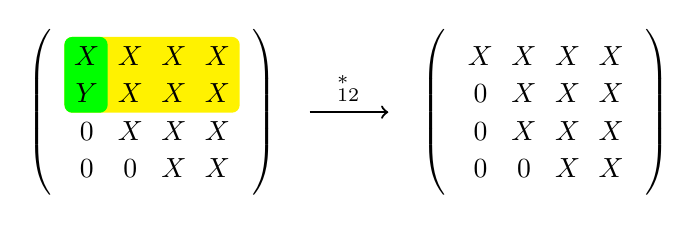
\begin{tikzpicture}\node
[matrix of math nodes,left delimiter=(,right delimiter=)] (m)  at (0,0)
{
  X&X&X&X\\
  Y&X&X&X\\
  0&X&X&X\\
  0&0&X&X\\
};

\node
[matrix of math nodes,left delimiter=(,right delimiter=)] (r)  at (5,0)
{
  X&X&X&X\\
  0&X&X&X\\
  0&X&X&X\\
  0&0&X&X\\
};

\draw[->,thick] (2,0) -- node[above] {$\matg_{12}^*\matH$} (3,0);

\begin{pgfonlayer}{bg}
  \node[fit={(m-1-1.north west) (m-2-4.south east)},fill=yellow,inner sep=0,rounded corners=1mm]{};
  \node[fit={(m-1-1.north west) (m-2-1.south east)},fill=green,inner sep=0,rounded corners=1mm]{};
\end{pgfonlayer}

;\end{tikzpicture}}
    \only<2>{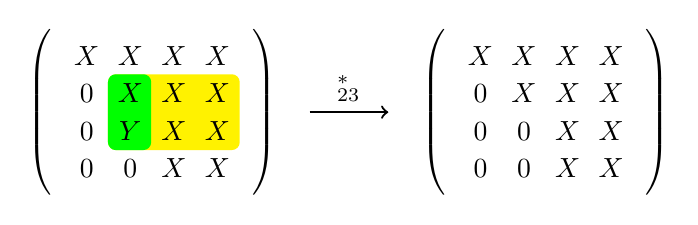
\begin{tikzpicture}\matrix
[matrix of math nodes,left delimiter=(,right delimiter=)] (m)
{
  X&X&X&X\\
  0&X&X&X\\
  0&Y&X&X\\
  0&0&X&X\\
};

\node
[matrix of math nodes,left delimiter=(,right delimiter=)] (r)  at (5,0)
{
  X&X&X&X\\
  0&X&X&X\\
  0&0&X&X\\
  0&0&X&X\\
};

\draw[->,thick] (2,0) -- node[above] {$\matg_{23}^*\matH$} (3,0);

\begin{pgfonlayer}{bg}
  \node[fit={(m-2-2.north west) (m-3-4.south east)},fill=yellow,inner sep=0,rounded corners=1mm]{};
  \node[fit={(m-2-2.north west) (m-3-2.south east)},fill=green,inner sep=0,rounded corners=1mm]{};
\end{pgfonlayer}
;\end{tikzpicture}}
    \only<3>{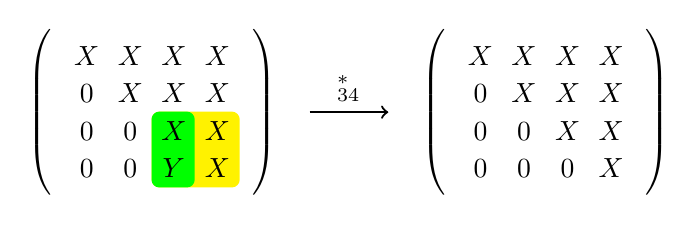
\begin{tikzpicture}\matrix
[matrix of math nodes,left delimiter=(,right delimiter=)] (m)
{
  X&X&X&X\\
  0&X&X&X\\
  0&0&X&X\\
  0&0&Y&X\\
};

\node
[matrix of math nodes,left delimiter=(,right delimiter=)] (r)  at (5,0)
{
  X&X&X&X\\
  0&X&X&X\\
  0&0&X&X\\
  0&0&0&X\\
};

\draw[->,thick] (2,0) -- node[above] {$\matg_{34}^*\matH$} (3,0);

\begin{pgfonlayer}{bg}
  \node[fit={(m-3-3.north west) (m-4-4.south east)},fill=yellow,inner sep=0,rounded corners=1mm]{};
  \node[fit={(m-3-3.north west) (m-4-3.south east)},fill=green,inner sep=0,rounded corners=1mm]{};
\end{pgfonlayer}
;\end{tikzpicture}}
    \only<4>{
      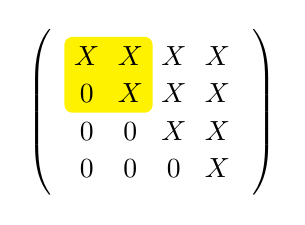
\begin{tikzpicture}\matrix
[matrix of math nodes,left delimiter=(,right delimiter=)] (m)
{
  X&X&X&X\\
  0&X&X&X\\
  0&0&X&X\\
  0&0&0&X\\
};
\begin{pgfonlayer}{bg}
  \node[fit={(m-1-1.north west) (m-2-2.south east)},fill=yellow,inner sep=0,rounded corners=1mm]{};
\end{pgfonlayer}
;\end{tikzpicture}
      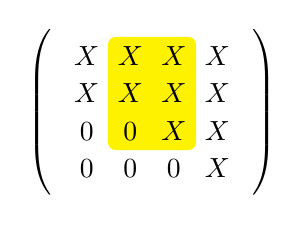
\begin{tikzpicture}\matrix
[matrix of math nodes,left delimiter=(,right delimiter=)] (m)
{
  X&X&X&X\\
  X&X&X&X\\
  0&0&X&X\\
  0&0&0&X\\
};
\begin{pgfonlayer}{bg}
  \node[fit={(m-1-2.north west) (m-3-3.south east)},fill=yellow,inner sep=0,rounded corners=1mm]{};
\end{pgfonlayer}
;\end{tikzpicture}
      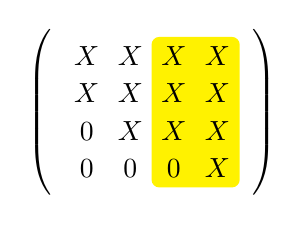
\begin{tikzpicture}\matrix
[matrix of math nodes,left delimiter=(,right delimiter=)] (m)
{
  X&X&X&X\\
  X&X&X&X\\
  0&X&X&X\\
  0&0&0&X\\
};
\begin{pgfonlayer}{bg}
  \node[fit={(m-1-3.north west) (m-4-4.south east)},fill=yellow,inner sep=0,rounded corners=1mm]{};
\end{pgfonlayer}
;\end{tikzpicture}
      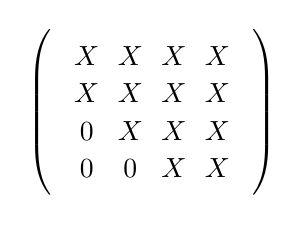
\begin{tikzpicture}\matrix
[matrix of math nodes,left delimiter=(,right delimiter=)] (m)
{
  X&X&X&X\\
  X&X&X&X\\
  0&X&X&X\\
  0&0&X&X\\
};
;\end{tikzpicture}}
  \end{frame}
\frame {\input {blocks/Theorem-Hessenberg-qr.tex}}
\frame {\input {blocks/Corollary-Hessenberg-qr.tex}}
\frame {\input {blocks/Theorem-Hessenberg-householder.tex}}

\frame {\input {blocks/Algorithm-qr-method.tex}}

\frame {\input {blocks/Theorem-hessenberg-qr-convergence.tex}}

\subsubsection{Deflation and shifts}
\frame {\input {blocks/Theorem-qr-reduction.tex}}
\frame {\input {blocks/Algorithm-qr-deflation.tex}}
\frame {\input {blocks/Definition-hessenberg-unreduced.tex}}
\frame {\input {blocks/Theorem-implicit-Q.tex}}

\frame {\input {blocks/Algorithm-shifted-qr-iteration.tex}
  \input {blocks/Lemma-shifted-qr-convergence.tex}}
\frame {\input {blocks/Lemma-perfect-shift.tex}}
\frame {\input {blocks/Example-rayleigh-shift.tex}}
\frame {\input {blocks/Definition-wilkinson-shift.tex}}
\frame {\input {blocks/Remark-wilkinson-shift.tex}}
\frame {\input {blocks/Algorithm-qr-deflation.tex}}

\subsection{Methods in real arithmetic}
\frame{\subtoc}
\subsubsection{The real symmetric EVP}
\frame{\subsubtoc}

\frame {\input {blocks/Lemma-qr-tridiagonal.tex}}
\frame {\input {blocks/Lemma-perfect-shift-sym.tex}}
\frame {\input {blocks/Remark-real-symmetric-qr.tex}}
\frame {\input {blocks/Algorithm-qr-explicit-shift.tex}}
\frame {\input {blocks/Lemma-wilkinson-shift.tex}}
\frame {\input {blocks/Notation-givens-specific.tex}
  \input {blocks/Algorithm-implicit-symmetric-shift.tex}}
\frame {\input {blocks/Theorem-implicit-symmetric-shift.tex}}

\subsubsection{The EVP for nonsymmetric real matrices}
\frame{\subsubtoc}
\frame {\input {blocks/Theorem-real-schur-form.tex}}
\frame {\input {blocks/Algorithm-double-shift-step.tex}}
\frame {\input {blocks/Lemma-double-shift-matrix.tex}}
\frame {\input {blocks/Theorem-implicit-double-shift.tex}}
\frame {\input {blocks/Algorithm-deflation-francis.tex}}

% \subsubsection{Singular Value Decomposition (SVD)}
% \frame{\subsubtoc}
% \frame {\input {blocks/Definition-svd.tex}
%   \input {blocks/Theorem-svd.tex}}
% \frame {\input {blocks/Corollary-svd-rank.tex}
%   \input {blocks/Corollary-svd-inverse.tex}}
% \frame {\input {blocks/Remark-svd-geometry.tex}}
% \frame {\input {blocks/Lemma-svd-ata.tex}}
% \frame {\input {blocks/Theorem-implicit-Q.tex}}

%%% Local Variables:
%%% mode: latex
%%% TeX-master: "slides"
%%% End:


\section{Solving Large Sparse Linear Systems}
\frame{\sectoc}

\subsection{Motivation and sparse matrices}
\frame {\input {blocks/Definition-sparse-matrix.tex}}
\frame {\input {blocks/Example-page-rank.tex}}
\frame {\input {blocks/Example-csr.tex}}
\frame {\input {blocks/Remark-algorithmic-matrix.tex}}

\subsection{Basic iterations}
\frame{\subtoc}
\frame {\input {blocks/Definition-jacobi.tex}
  \input {blocks/Definition-gauss-seidel.tex}}
\frame {\input {blocks/Definition-richardson-iteration.tex}}
\frame {\input {blocks/Definition-matrix-iteration.tex}}
\frame {\input {blocks/Lemma-Jacobi-gs-matrices.tex}}

\frame {\input {blocks/Theorem-bfpt.tex}}
\frame {\input {blocks/Corollary-bfp-estimates.tex}}
\frame {\input {blocks/Corollary-matrix-norm-convergence.tex}}
\frame {\input {blocks/Example-convergence-row-sum.tex}}
\frame {\input {blocks/Example-matrix-norm-convergence.tex}}

\frame {\input {blocks/Definition-spectral-radius.tex}}
\frame {\input {blocks/Lemma-spectral-radius.tex}}
\frame {\input {blocks/Theorem-matrix-radius-convergence.tex}}
\frame {\input {blocks/Remark-contraction-vs-convergence.tex}}
\frame {\input {blocks/Theorem-richardson-convergence.tex}}
\frame {\input {blocks/Remark-richardson-convergence.tex}}
\frame {\input {blocks/Definition-convergence-rate-logarithmic.tex}}


%%% Local Variables:
%%% mode: latex
%%% TeX-master: "slides"
%%% End:

\subsection{Projection methods}
\frame{\subtoc}
\subsubsection{Review of projection operators}
\frame {\input {blocks/Definition-projection.tex}}
\frame {\input {blocks/Lemma-projection-complement.tex}}
\frame {\input {blocks/Lemma-projection-spaces.tex}}
\frame {\input {blocks/Definition-projection-spaces-orthogonal.tex}
  \input {blocks/Lemma-projection-spaces-orthogonal.tex}}
\frame {\input {blocks/Definition-biorthogonal.tex}}
\frame {\input {blocks/Lemma-projection-basis.tex}}

\subsubsection{Galerkin methods}
\frame{\subsubtoc}
\frame {\input {blocks/Definition-galerkin-method.tex}}
\frame {\input {blocks/Definition-projection-step.tex}}
\frame {\input {blocks/Example-projection-gauss-seidel.tex}}

\frame {\input {blocks/Definition-projection-method-matrix.tex}}
\frame {\input {blocks/Theorem-projected-invertible.tex}}
\frame {\input {blocks/Theorem-projection-orthogonal-optimal.tex}}
\frame {\input {blocks/Theorem-projection-oblique-optimal.tex}}

\subsubsection{Steepest descent and minimal residual algorithms}
\frame{\subsubtoc}
\frame {\input {blocks/Example-projection-1d.tex}}
\frame {\input {blocks/Algorithm-steepest-descent-algol.tex}
  \input {blocks/Lemma-steepest-descent.tex}}
\frame {\input {blocks/Remark-convergence-residual.tex}}
\frame {\input {blocks/Algorithm-steepest-descent-python1.tex}}
\frame {\input {blocks/Algorithm-steepest-descent-python2.tex}}
\frame {\input {blocks/Algorithm-minimal-residual-algol.tex}
  \input {blocks/Lemma-minimal-residual.tex}}
\begin{frame}
  \begin{columns}
    \begin{column}{.48\textwidth}
      \input {blocks/Algorithm-steepest-descent-algol.tex}
    \end{column}
    \begin{column}{.48\textwidth}
      \input {blocks/Algorithm-minimal-residual-algol.tex}
    \end{column}
  \end{columns}
\end{frame}
\frame {\input {blocks/Lemma-lucky-breakdown.tex}}
\frame {\input {blocks/Lemma-kantorovich-inequality.tex}}
\frame {\input {blocks/Theorem-steepest-descent-convergence.tex}}
\frame {\input {blocks/Theorem-minimal-residual-convergence.tex}}

\subsection{Krylov space methods}
\frame{\subtoc}
\frame {\input {blocks/Definition-krylov-space.tex}}
\frame {\input {blocks/Definition-grade-of-v.tex}}
\frame {\input {blocks/Lemma-krylov-polynomial.tex}}
\frame {\input {blocks/Lemma-krylov-projector.tex}}

%%% Local Variables:
%%% mode: latex
%%% TeX-master: "slides"
%%% End:

\subsubsection{The Arnoldi and Lanczos processes}
\frame{\subsubtoc}
\frame {\input {blocks/Lemma-Hessenberg-Krylov-1.tex}}
\frame {\input {blocks/Theorem-arnoldi-projection.tex}}
\frame {\input {blocks/Theorem-Hessenberg-Krylov-2.tex}
  \pause
  \input {blocks/Corollary-Hessenberg-Krylov.tex}}
\frame {\input {blocks/Algorithm-arnoldi-1.tex}}

\frame {\input {blocks/Lemma-arnoldi-w.tex}}
\frame {\input {blocks/Notation-arnoldi-step.tex}
  \input {blocks/Lemma-arnoldi-breakdown.tex}}

\frame {\input {blocks/Lemma-arnoldi-symmetric.tex}}
\frame {\input {blocks/Algorithm-lanczos.tex}}

%%% Local Variables:
%%% mode: latex
%%% TeX-master: "slides"
%%% End:

\subsubsection{Lanczos process and cg}
\frame{\subsubtoc}
\frame {\input {blocks/Lemma-arnoldi-symmetric.tex}}
\frame {\input {blocks/Algorithm-lanczos.tex}}

\frame {\input {blocks/Theorem-arnoldi-linear-system.tex}}
\frame {\input {blocks/Theorem-arnoldi-linear-residual.tex}}

\frame {\input {blocks/Lemma-lanczos-linear.tex}}
\frame {\input {blocks/Lemma-lanczos-incremental.tex}}
\frame {\input {blocks/Lemma-lanczos-orthogonality.tex}}
\frame {\input {blocks/Algorithm-cg.tex}}
\frame {\input {blocks/Lemma-cg-orthogonality.tex}}

\frame {\input {blocks/Theorem-projection-orthogonal-optimal.tex}}
\frame {\input {blocks/Lemma-krylov-polynomial.tex}}

\frame {\input {blocks/Theorem-cg-optimality.tex}
  \pause
  \input {blocks/Corollary-cg-vs-descent}}
\frame {\input {blocks/Corollary-cg-optimality-spectrum.tex}}

\frame {\input {blocks/Definition-chebyshev-polynomials.tex}}
\frame {\input {blocks/Lemma-chebyshev-representation.tex}}
\frame {\input {blocks/Lemma-chebyshev-abscissae.tex}}
\frame {\input {blocks/Theorem-chebyshev-minimal-1.tex}}
\frame {\input {blocks/Lemma-chebyshev-growth.tex}}
\frame {\input {blocks/Corollary-chebyshev-minimal-2.tex}}
\frame {\input {blocks/Corollary-cg-condition-number.tex}}

%%% Local Variables:
%%% mode: latex
%%% TeX-master: "slides"
%%% End:

\subsubsection{Lanczos Biorthogonalization}
\frame{\subsubtoc}
\frame {\input {blocks/Lemma-projection-basis.tex}}
\frame {\input {blocks/Algorithm-bi-lanczos.tex}}
\frame {\input {blocks/Theorem-bi-lanczos-projection.tex}}

\subsubsection{Preconditioning}
\frame{\subsubtoc}
\frame {\input {blocks/Definition-preconditioned-system.tex}}
\frame {\input {blocks/Definition-preconditioner.tex}}
\frame {\input {blocks/Lemma-preconditioner-symmetry}
  \pause
  \input {blocks/Algorithm-lanczos.tex}}
\frame {\input {blocks/Algorithm-pcg.tex}}



\section{Large Sparse Eigenvalue Problems}
\frame{\sectoc}

\subsection{Projected subspace iteration}
\frame {\input {blocks/Definition-galerkin-ev.tex}}
\frame {\input {blocks/Algorithm-rayleigh-ritz.tex}}
\frame {\input {blocks/Definition-ritz-values.tex}}
\frame {\input {blocks/Lemma-ritz-invariant.tex}}
\frame {\input {blocks/Lemma-Courant-Fischer-Ritz.tex}}
\frame {\input {blocks/Lemma-ritz-rayleigh-estimate.tex}}
\frame {\input {blocks/Lemma-ritz-estimate-sine.tex}}

\frame {\input {blocks/Algorithm-ev-projection.tex}}
\frame {\input {blocks/Definition-ritz-values.tex}}
\frame {\input {blocks/Theorem-ritz-convergence.tex}}

\subsection{The Lanczos method}
\frame{\subtoc}

\frame {\input {blocks/Algorithm-lanczos.tex}}
\frame {\input {blocks/Algorithm-ev-lanczos.tex}}
\frame {\input {blocks/Algorithm-cg.tex}}
\frame {\input {blocks/Lemma-cg-tridiagonal.tex}}
\frame {\input {blocks/Lemma-lanczos-angle.tex}}
\frame {\input {blocks/Theorem-lanczos-angle.tex}}
\frame {\input {blocks/Theorem-lanczos-eigenvalue-estimate.tex}}

%%% Local Variables:
%%% mode: latex
%%% TeX-master: "slides"
%%% End:

\subsection{The Arnoldi method}
\frame{\subtoc}

\frame {\input {blocks/Algorithm-ev-arnoldi.tex}}
\frame {\input {blocks/Definition-arnoldi-factorization.tex}}
\frame {\input {blocks/Lemma-ev-arnoldi-a-posteriori.tex}
  \input {blocks/Corollary-ev-arnoldi-breakdown.tex}}
\frame {\input {blocks/Definition-arnoldi-locking.tex}}
\frame {\input {blocks/Definition-polynomial-filtering.tex}}
\frame {\input {blocks/Lemma-filtering-restart.tex}}
\frame {\input {blocks/Algorithm-implicit-restart.tex}}
\frame {\input {blocks/Algorithm-iram.tex}}
% \frame {\input {blocks/Theorem-arnoldi-projection.tex}}
% \frame {\input {blocks/Lemma-perfect-shift.tex}}
% \frame {\input {blocks/Lemma-arnoldi-truncation.tex}}
\frame {\input {blocks/Algorithm-arnoldi-reorthogonalization}}

%%% Local Variables:
%%% mode: latex
%%% TeX-master: "slides"
%%% End:


\section{Programming exam}
\frame{\sectoc}


\begin{frame}
  \begin{block}{Assignment}
    Implement the QR-method with shifts and deflation for Hermitian
    matrices and document the decisions you made in the implementation.
    
    Verify your program with meaningful tests and document their results.
  \end{block}
\end{frame}

\begin{frame}
  \frametitle{Formalities}
  \begin{itemize}
  \item The program(s), documentation, and results should be submitted
    electronically in a single PDF by Feb 6th, 2023.
  \item You are welcome and encouraged to discuss your work with your
    peers, but every student must submit their own, unique work.
  \item  As part of the exam, you will be asked to give a short oral
    presentation of your work and you should be able to answer questions
    about your code.
  \item Oral presentations will be scheduled for the week of
    Feb 6th, or later upon request.
  \end{itemize}
\end{frame}

\begin{frame}
  \frametitle{Guidelines}
  \begin{enumerate}
  \item The program must run with several example matrices without
    crashing and you must be able to change parameters like the matrix
    size
  \item The program must be subdivided into functions of well-defined
    purpose
  \item Your code should be well structured and readable
  \item You must be able to describe how you verify the correctness of
    your program
  \item Follow all suggestions from the notes on how to save memory and operations
  \item Avoid complex numbers whenever possible
  \item The QR iteration must be able to identify multiple eigenvalues
  \item Use appropriate shift strategies and document
  \item Document your deflation strategy
  \item Bonus if you compute not only eigenvalues but also eigenvectors
  \end{enumerate}
\end{frame}

\begin{frame}
  \frametitle{Hints}
  \begin{enumerate}
\item Jupyter notebooks are a great way of producing this PDF, but
  they are not necessary.
\item The ``[:]'' notation for selecting column vectors or submatrices
  can be very helpful, if used the right way.
\end{enumerate}
\end{frame}

\frame {\input {blocks/Algorithm-householder-multiplication.tex}}
\frame {\input {blocks/Algorithm-givens-multiplication.tex}}
\frame {\input {blocks/Problem-Hermitian-tridiagonal.tex}}
\frame {\input {blocks/Remark-tridiagonal-storage.tex}}


%%% Local Variables:
%%% mode: latex
%%% TeX-master: "slides"
%%% End:


\section*{Bibliography}
\frame{\bibliographystyle{alpha}
\bibliography{all}}

%\frame {\input {blocks/Satz-trigonometrische-interpolation.tex}}

\end{document}

%%% Local Variables:
%%% mode: latex
%%% TeX-master: t
%%% End:
